\documentclass[twocolumn]{article}

\usepackage{amsmath, amssymb}
\usepackage{natbib}
\usepackage{subcaption}
\usepackage{graphicx}
\usepackage{color}
\usepackage{hyperref}
\usepackage{enumitem}
\setitemize{noitemsep,topsep=0pt,parsep=0pt,partopsep=0pt}

\title{Avoiding Flight Delays with Supervised Ranking}
\author{Dan Garant \and John Lalor \and Adam Nelson}
\date{}

\begin{document}
\maketitle

\begin{abstract}
In this work, we examine the task of selecting flights to minimize the risk of encountering a flight delay.
Taking the perspective of a passenger attempting to book a flight one day in advance or thirty days in advance, we gather and explore a number weather, airport, and air carrier characteristics that can be used to assess the probability of experiencing a delay.
For each time horizon under consideration, these features vary in availability and quality, yielding an interesting pair of machine learning tasks.
We evaluate a number of supervised learning models for each task, and present results in the form of rankings, consistent with a strategy that could be employed by a flight-booking service.
\end{abstract}

\section{Introduction}

In recent years, the U.S. Bureau of Transportation Statistics (BTS)  has enabled easy access to a wealth of information on on-time flight performance of domestic air carriers\footnote{\url{http://www.transtats.bts.gov/}}.
Given the availability of flight characteristics, the task of determining whether a flight will take off and arrive on time is well-suited for analysis with machine learning.
Air transportation has become a central aspect of the U.S. culture for both business and recreation, with the number of domestic flights offerings growing steadily for decades.
Accompanying the growth in air travel, numerous online services including Google Flights and Expedia provide passengers the ability to select from a variety of available air carriers, flight dates, and origins, when booking a flight.
However, these services provide only high-level historic information about carrier-specific patterns in delays, if at all.

Combining historical characteristics of air carriers and airports with weather forecasts and weather trends (or \emph{normals}) would enable flight booking sites to provide more reliable and targeted information about delay risk.
Our objective is to use supervised learning models to identify the flights with a low probability of delay. Our analysis will look at flight delay patterns according to two distinct problems: predicting a flight delay for flights leaving tomorrow, and predicting flight delays for flights leaving in thirty days.
In section~\ref{sec:data-sources}, we give an overview of the BTS dataset, previous studies or airline delays using this dataset, and supplemental weather data sources we employ.
In section~\ref{sec:exploratory}, we examine patterns in delays that can be exploited to construct a probabilistic model of delays.
Section~\ref{sec:evaluation-methodology} formally details our method of evaluation, and section~\ref{sec:results} explores the results obtained by many commonly-used supervised learning models of various levels of sophistication.
\section{Data Sources}

\label{sec:data-sources}
\subsection{Bureau of Transportation Dataset}

The original idea for the project came from the 2009 American Statistical Association Joint Statistical Meetings Data Expo \citep{wickham2011asa}.
The challenge was to create a graphical summary of the data, which consisted of flight statistics from October 1987 to April 2008.
The submissions for this explored a variety of aspects of the data, a number of which are mentioned below.

The data for the 2009 ASA Expo came from the United States Department of Transportation (DOT).
The DOT Bureau of Transportation Statistics (BTS) track flight statistics for domestic flights. 
For the purposes of our project, we focused on flight statistics from the year 2014, as these flights were more recent than the original expo dataset and still provide a large set of data from which we could obtain conclusions. 
We obtained the data directly from the BTS website.

The BTS data includes a large number of data fields. Below we enumerate the fields that we included in our analysis, along with a description of each:

\begin{itemize}
\item Origin Airport and Departure Airports: Origin and departure airports for each flight in the dataset, encoded as a discrete characteristic with one-hot encoding. 250 airports were represented in this dataset.
\item Month, Day of Month, and Day of Week: Included since traffic patterns vary over the course of the year---specific periods could be tied to flight delays. Month and day of week were encoded as discrete characteristics.
\item Carrier: Discrete characteristic representing the carrier of the flight. 14 distinct carriers were represented in the data.
\item Scheduled Departure and Arrival Time: Scheduled arrival and departure times for each flight, as provided by the Computer Reservation System (CRS) used by travel agents to allow agents to book flights and issue tickets.
\item Distance: Distance from the origin to the destination
\item Airport volume in and out: For each flight, we calculated the number of other flights scheduled to arrive and depart within the same hour that the reference flight was scheduled to depart. 
\end{itemize}

\subsection{Related Work}

As part of the 2009 task, there were a number of submissions that used the dataset in interesting ways. We will briefly discuss the top four submissions for that task here.
\cite{wicklin2009congestion} used SAS Software to provide a number of visualizations of the data, including departure delay heatmaps by month for each of the years included in the data and historical comparisons of flight delays, showing that the number of delays varied widely between years.
\cite{hofmann2011delayed} found that Newark airport was the worst offender when it came to flight delays, which one author can back up empirically.
\cite{wickham2011tale} looked at two specific airports, Oakland and San Francisco, and compared number of flights between the two airports, looking at trends in flight numbers in the two airports.
\cite{dey2009minimizing} modeled the data as a graph in order to predict delays for any origin-destination pair.

In addition to work performed as part of the 2009 Expo, there has been additional work using the BTS data.
\cite{rupp2006does} investigated whether competition for specific routes influences airline performance and found that \emph{busy} routes (that is, routes with a number of carriers) tend to have more delays.
\cite{stone2015investigating} found that small community airports suffered from departure delays, which then had a large effect on those passengers missing connecting flights and incurring large costs for rebooking.


\subsection{Supplemental Data}

In addition to the data provided by the BTS, we augmented the feature set for flights with weather forecasts and patterns for each of the airports to determine the effect that weather might have on flight delays.
For our two tasks, this involved obtaining two new sets of features: detailed weather information for the one-day task, and high level weather normals for the one-month task.

The intuition here was that if you are looking to predict flight delays for tomorrow's flights, a lot of detailed weather information will be available for tomorrow that is most likely very accurate.
One month in advance, however, the weather information is less likely to be accurate, so we instead looked at ten-year normals for the flight dates, in order to get an idea of weather one month in advance.
Therefore in order to effectively simulate the amount of data available to a model when dealing with our two task scenarios, we only included the detailed flight information in our one-day feature set, and only included the high-level weather normals in our thirty-day task feature set.


In case of the one-day task, a wealth of relatively accurate and detailed weather information is available. We gathered historical weather data for a about 50\% of 2014 flights represented in the BTS data using a popular weather API\footnote{\url{https://developer.forecast.io/}}. This API provided 12 features:
\begin{itemize}
\item Precipitation intensity, measured in inches per hour
\item Recent precipitation intensity, a derived feature, which we computed as the mean of precipitation intensity values for the previous 3 hours
\item Dew point
\item Visibility in miles
\item Temperature
\item Apparent temperature, representing a ``feels like'' temperature
\item Pressure in millibars
\item Precipitation probability, when actual precipitation data is not available but a forecast is
\item Humidity
\item Wind speed in miles per hour
\item Wind bearing, ranging from 0 to 359 with 0 indicating that the wind is blowing true north
\item Weather summary, a concise summary of the weather which we represented as a discrete characteristic
\end{itemize}

In the case of the one-month task, quality weather forecasts are not avilable. Historical weather data would be inappropriate to include, so instead we collected ten-year climate normals for the flight dates from the National Oceanic and Atmospheric Administration (NOAA) National Centers for Environmental Information (NCEI) \citep{noaaclimatedata}.  For our task, we looked at the temperature normals collected over a period of years, from 1981 to 2010. Specifically, we used the high, low, and average temperature for both origin and destination airports.

\section{Exploratory Analysis}
\label{sec:exploratory}

To inform our selection and tuning of supervised learning algorithms for this task, we performed a number of exploratory analyses characterizing the nature of dependence between specific features and the response (departure delay in minutes). First, we investigated characteristics of organizations involved in fulfilling the flight. Using a linear model, we estimated the conditional mean and variance of the departure delays (in minutes) given air carrier. We find significant differences between carriers, shown in Figure~\ref{fig:carrier-performance}. Southwest Airlines is the biggest offender, with an expected delay duration of more than 15 minutes. At the other end of the spectrum, Hawaiian Airlines has a negative expectation, indicating that most flights leave before scheduled.

\begin{figure*}
    \centering
    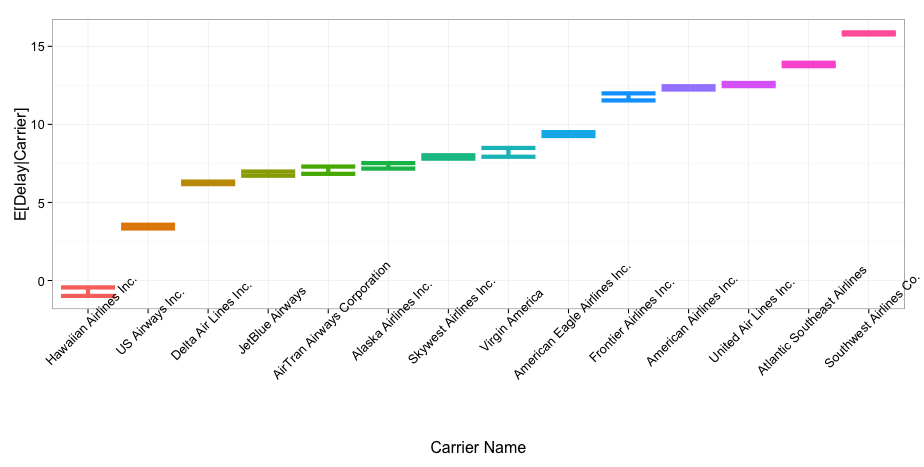
\includegraphics[width=\linewidth]{figures/carrier-performance.png}
    \caption{Performance of Major Domestic Air Carriers}
    \label{fig:carrier-performance}
\end{figure*}

To gain a high-level understanding of the relationship between the weather features and delays, we fit a generalized additive model \citep{hastie1990generalized} of delay duration (in minutes) to a linear combination of cubic spline transformations of various weather features. Naturally, there are associations between each of the weather characteristics. For instance, humidity will necessarily be high when it is raining. To isolate the \emph{independent} effects of each of the features on the departure delay, we predicted the conditional expectation of delay $D$ with respect to an individual feature $X_i$, holding other features at their mean value:
\begin{align}
    \label{eq:conditional-exp}
    E[D|X_1=\bar{X_1}, X_2=\bar{X_2}, \ldots, X_i = x_i, \ldots, X_n = \bar{X_n}].
\end{align}
Then, sweeping across various settings for $x_i$ and various feature $X_i$ yields a sensible explanatory model of delay with respect to weather characteristics. When stratifying by airport and evaluating (\ref{eq:conditional-exp}) with respect to wind bearing, we find a strong non-linear relationship illustrated in Figure~\ref{fig:wind-bearing-feature}. 
This dependence is likely the result of differing runway orientation at various airports. When wind is blowing \emph{across} a runway, take-off and landing is more challenging, and some pilots may opt to defer until winds are more favorable. Each airport may have a different runway orientation, so the model must be capable of capturing interactions between a discrete characteristic (airport) and a real-valued characteristic (wind direction).
We also find intuitive dependencies between precipitation intensity, shown in Figure~\ref{fig:precip-delay-relationship}, and wind speed, shown in Figure~\ref{fig:wind-speed-delay-relationship}.

\begin{figure*}
\centering
\begin{subfigure}{0.45\textwidth}
    \centering
    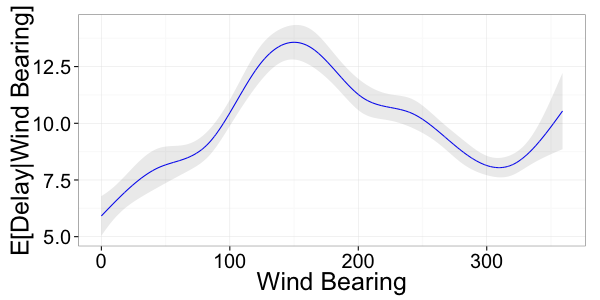
\includegraphics[width=\linewidth]{figures/windBearing-ATL.png}
    \caption{Hartsfield-Jackson Atlanta}
\end{subfigure}
\begin{subfigure}{0.45\textwidth}
    \centering
    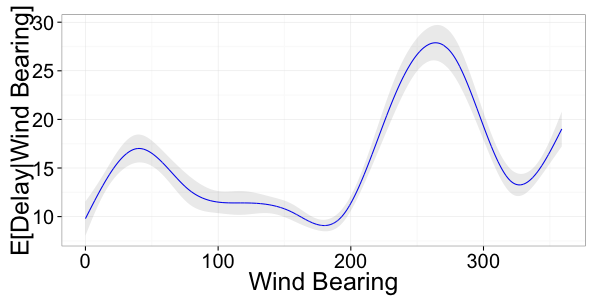
\includegraphics[width=\linewidth]{figures/windBearing-DFW.png}
    \caption{Dallas/Fort Worth}
\end{subfigure}
\caption{Relationship between wind bearing and expected delays (in minutes) at various airports. One standard error in the conditional expectation is shown in gray.} 
\label{fig:wind-bearing-feature}
\end{figure*}

\begin{figure*}
    \centering
\begin{subfigure}{0.45\textwidth}
    \centering
    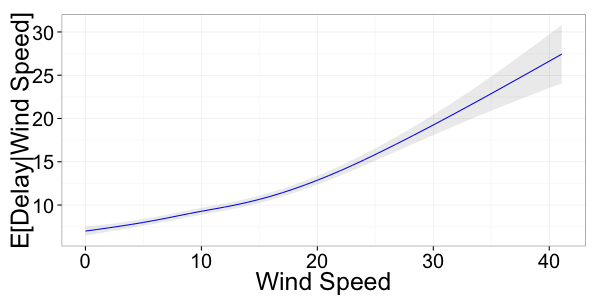
\includegraphics[width=\linewidth]{figures/windSpeed.png}
    \caption{Relationship between wind speed and delay}
    \label{fig:wind-speed-delay-relationship}
\end{subfigure}
\begin{subfigure}{0.45\textwidth}
    \centering
    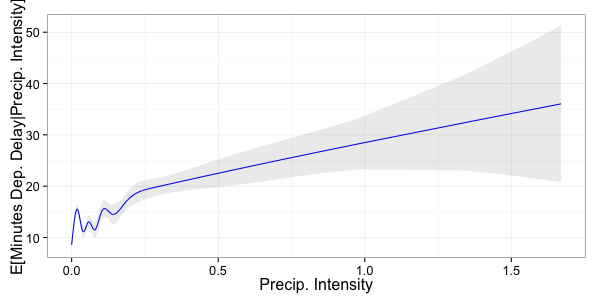
\includegraphics[width=\linewidth]{figures/precipIntensity.png}
    \caption{Relationship between precipitation and delay}
    \label{fig:precip-delay-relationship}
\end{subfigure}
\end{figure*}

\begin{figure}
\end{figure}


\section{Evaluation Methodology}
\label{sec:evaluation-methodology}

In this work, we considered evaluating according to two related but distinct tasks: delay classification and risk ranking. In both cases, the training data consists of set of 3,500 flights randomly sampled from all 2014 flights for which weather data was available. Each flight is annotated with a binary delay class, ``delay'' if the flight left 1 or more minute after the scheduled departure time, or ``no delay'' otherwise. For the delay classification task, learning algorithms are evaluated based on how well they can predict this binary class label. From a distinct pool of 1,500 test flights, we compute the classification accuracy as the proportion of correctly labeled instances.

The risk ranking task is more closely related to the intended passenger-centric use case. For this task, the test set consists of 750 \emph{pairs} of flights, where each pair has the same origin, destination, and flight date. For each flight in the pair, the delay probability, $P(D=\text{delay}|x_1, x_2, x_3, \ldots, x_n)$, is estimated, rather than the delay class. The flight with the smallest delay probability is marked as ``favorable''. Then, the ranking accuracy is computed as the proportion of pairs for which (1) the pair has differing delay status, and (2) the favorable flight experienced a shorter delay.

\begin{figure*}
    \centering
    \begin{subfigure}{0.45\textwidth}
        \centering
        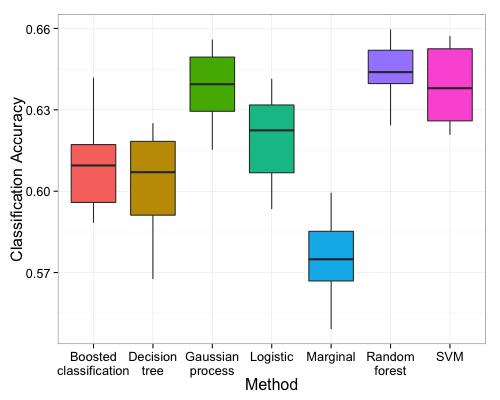
\includegraphics[width=\linewidth]{figures/class-performance-sample-5000-OneDayHorizon.png}
        \caption{One-day horizon}
    \end{subfigure}
    \begin{subfigure}{0.45\textwidth}
        \centering
        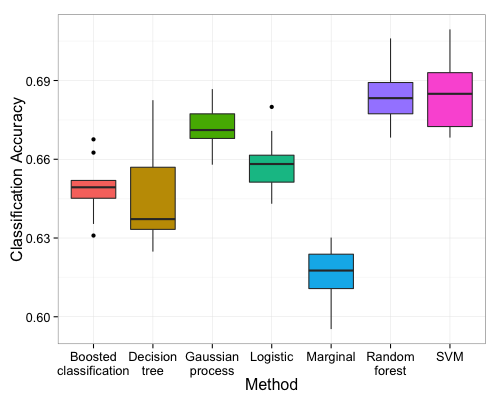
\includegraphics[width=\linewidth]{figures/class-performance-sample-5000-OneMonthHorizon.png}
        \caption{Thirty-day horizon}
    \end{subfigure}
    \caption{Classification Accuracy}
    \label{fig:classification-accuracy}
\end{figure*}

\begin{figure*}
    \centering
    \begin{subfigure}{0.45\textwidth}
        \centering
        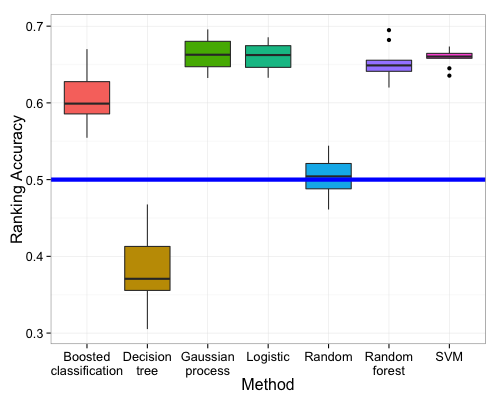
\includegraphics[width=\linewidth]{figures/performance-sample-5000-OneDayHorizon.png}
        \caption{One-day horizon}
    \end{subfigure}
    \begin{subfigure}{0.45\textwidth}
        \centering
        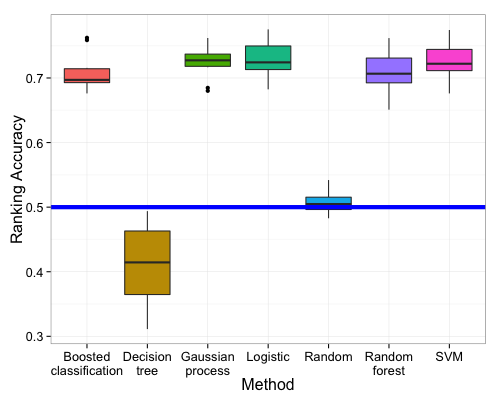
\includegraphics[width=\linewidth]{figures/performance-sample-5000-OneMonthHorizon.png}
        \caption{Thirty-day horizon}
    \end{subfigure}
    \caption{Ranking Accuracy}
    \label{fig:ranking-accuracy}
\end{figure*}

We considered machine learning algorithms from three categories:
\begin{itemize}
    \item Simple/baseline methods: These included methods that predict from marginal and uniformly random class probabilities. The marginal baseline represents a ``null'' model for the delay classification task. It always predicts the most common class. The uniform random baseline represents a null model for the ranking task, as it randomly marks one of the flights as favorable. We also considered classical logistic regression.
    \item Tree-based methods: This category includes decision trees, random forests, and boosted classification trees. We tuned the complexity penality of decision trees with linear search. For random forests, we set set the number of trees with cross-validation, and for boosted classification trees, we set the number of boosting iterations with cross-validation.
    \item Kernel-based methods: In this group, we used support vector machines and Gaussian processes. In each case, we used a radial basis function kernel with bandwidth hyper-parameter set with linear search.
\end{itemize}

\section{Results}
\label{sec:results}

Figure~\ref{fig:classification-accuracy} shows the performance of classification results for both the one-day and thirty-day tasks. Several properties are apparent. First, all of the methods are able to generally out-perform the marginal baseline. In both cases, support vector machines and random forests are most effective. With the exception of random forests, tree-based methods perform rather poorly, perhaps owing to the relatively high cardinality of discrete features such as airport and carrier. Interesting, performance in the one-day task is comparable to that in the one-month task. This suggests that weather information is relatively uninformative in predicting delays. Upon inspecting the distribution of weather characteristics during the hour that all 2014 flights were scheduled to depart, we found that 91\% of instances are categorized as clear, partly cloudy, mostly cloudy, or overcast. Even while the ratio of clear to rainy days in the U.S. is approximately 3:1, the number of \emph{hours} without precipitation to those with precipitation is approximately 20:1. Thus, while there is a strong relationship between various forms of inclement weather, as shown in section~\ref{sec:exploratory}, opportunities to exploit this information are fairly limited.

Figure~\ref{fig:ranking-accuracy} shows the results for the ranking task. In this case, the performance of most methods is fairly comparable, typically 10-20\% more accurate than random. Again, the additional weather information available in the one-day horizon task does not improve performance.

\section{Conclusion}
With this project we attempted to answer the following question: Can a machine learning model be used to identify a flight with the lowest probability of delay? 
Our motivation was from the point of view of an airline passenger. 
If someone needs to book a flight, they would like to book the flight with the lowest chance of delay.
Our project looked at two different flight-booking scenarios, booking a flight tomorrow and booking a flight in a month's time.
For these two tasks we combined flight data with relevant weather data, and found that a number of machine learning methods were able to outperform a base marginal classifier.
Future work could include looking at more complex patterns in the flight data, including multiple delays in a day at a particular airport or particular multi-location routes that are more or less likely to have delays.



\bibliographystyle{named}
\bibliography{bibliography}

\end{document}

